\section{What a single basepoint sees}\label{tf:sec:window}

Theorem~\ref{tf:thm:deconv}, like Lagarias's criterion \cite{Lagarias} (Remark~\ref{rem:ch2:oneline}), needs every level. A test at one level $\varepsilon$ sees less, and Section~\ref{sec:ch13:visibility}, with its Table~\ref{tab:ch13:see} and Exercise~\ref{ex:ch15:beside}, sets out what it sees in a lattice model. Two facts frame it. A zero at distance $\delta=\beta-\tfrac12>0$ from the line contributes positively at every level $\varepsilon>\delta$, so those levels cannot see it. As $\varepsilon\uparrow\delta$ its contribution at $\theta=\gamma$ is $-1/(\pi(\delta-\varepsilon))\to-\infty$, so the levels just below $\delta$ always see it. Near the line the test reduces to the sign of Laguerre's quantity $\mathcal L_\Xi=-(\log|\Xi|)''$.

A quadruple of zeros $\tfrac12\pm\delta\pm i\gamma^*$ with $\delta>0$ is added by hand to quantities computed from the actual zeros, to $\xi'/\xi$ and to $\mathcal L_\Xi$, in the way that Section~\ref{ag:sec:num} inserts quadruples into the computed density, and nothing below says that $\xi$ has such zeros. The tables, the figures and Corollary~\ref{tf:cor:levels} describe what a test would see if it did, and are statements about a model. A quadruple puts two zeros in the upper half plane, and it is placed among the actual zeros in one of three ways, which differ in the number of zeros up to a given height:
\begin{enumerate}
\item[(i)] the quadruple replaces one on line zero, at the ordinate $\gamma^*$ of that zero, as in the lattice of Section~\ref{sec:ch13:visibility}; the count of zeros up to a given height above $\gamma^*$ grows by one;
\item[(ii)] the quadruple is inserted at the midpoint $\gamma^*$ of a gap between consecutive on line zeros; the count grows by two;
\item[(iii)] the quadruple replaces the two on line zeros that bound a gap and sits at the midpoint $\gamma^*$ of the gap, as in the perturbation of Theorem~\ref{thm:ch13:perturb}; the count is unchanged.
\end{enumerate}


\begin{proposition}[The test near the line]\label{tf:prop:nearline}
Let $\theta$ be real and not the ordinate of a zero on the line, and let $\rho_\varepsilon(\theta)=\pi^{-1}\re(\xi'/\xi)(\tfrac12+\varepsilon+i\theta)$, defined by the same formula for every real $\varepsilon$. Then
\[
\rho_\varepsilon(\theta)=\frac{\varepsilon}{\pi}\,\mathcal L_\Xi(\theta)+O(\varepsilon^3)\quad(\varepsilon\to0),
\]
where
\[
\mathcal L_\Xi(\theta)=-\frac{d^2}{d\theta^2}\log|\Xi(\theta)|=\sum_\rho\frac{1}{(\theta-\gamma_\rho)^2},
\]
$\gamma_\rho=-i(\rho-\tfrac12)=\gamma-i(\beta-\tfrac12)$ are the zeros of $\Xi$, and the sum is real, since the zeros of $\Xi$ come in conjugate pairs. Under RH, $\mathcal L_\Xi(\theta)=\sum_\gamma(\theta-\gamma)^{-2}>0$. A quadruple of zeros $\tfrac12\pm\delta\pm i\gamma^*$ contributes
\[
2\re\frac{1}{(\theta-\gamma^*+i\delta)^2}+2\re\frac{1}{(\theta+\gamma^*+i\delta)^2},
\]
which equals $-2/\delta^2+O(\gamma^{*-2})$ at $\theta=\gamma^*$.
\end{proposition}

\begin{proof}
As a function of $(\theta,\varepsilon)$, $\rho_\varepsilon(\theta)$ is harmonic off the zeros and odd in $\varepsilon$ by the functional equation, so near $(\theta,0)$ it equals $\varepsilon\,\partial_\varepsilon\rho_\varepsilon(\theta)|_{\varepsilon=0}+O(\varepsilon^3)$. With $F=\xi'/\xi$ and $\Xi'(\theta)=iF(\tfrac12+i\theta)\Xi(\theta)$, differentiating gives $F'(\tfrac12+i\theta)=-(\Xi'/\Xi)'(\theta)$, which is real, and $\partial_\varepsilon\rho_\varepsilon=\pi^{-1}\re F'$. Hadamard's product for $\Xi$, with the zeros $\pm\gamma_\rho$ paired, gives $\Xi'/\Xi=\sum(\theta-\gamma_\rho)^{-1}$, and differentiating once more gives the sum. For the quadruple the zeros of $\Xi$ are $\gamma^*\pm i\delta$ and $-\gamma^*\pm i\delta$, and each conjugate pair contributes $2\re(\theta\mp\gamma^*+i\delta)^{-2}$; at $\theta=\gamma^*$ the first is $2\re(i\delta)^{-2}=-2/\delta^2$.
\end{proof}

At first order the test at $\gamma^*$ sees the quadruple exactly when
\[
\delta<\delta_c(\gamma^*)=\sqrt{2/\mathcal L_0(\gamma^*)},
\]
with $\mathcal L_0(\gamma^*)$ the contribution of the other zeros to $\mathcal L_\Xi(\gamma^*)$; this is the local visibility condition of Section~\ref{sec:ch13:visibility}, written with Laguerre's quantity. In (i) $\mathcal L_0$ omits the replaced zero; with neighbours at the mean spacing $\Delta=2\pi/\log(h/2\pi)$ this gives $\mathcal L_0=\pi^2/(3\Delta^2)$ and $\delta_c=(\sqrt6/\pi)\Delta=0.780\,\Delta$. In (ii), midway between two on line zeros, $\mathcal L_0=\pi^2/\Delta^2$ and $\delta_c=(\sqrt2/\pi)\Delta=0.450\,\Delta$. In (iii) the two zeros at $\gamma^*\pm\tfrac12\Delta$ are removed from the lattice of (ii), $\mathcal L_0=(\pi^2-8)/\Delta^2$ and $\delta_c=\sqrt{2/(\pi^2-8)}\,\Delta=1.034\,\Delta$. A distance $\delta_c=c\Delta$ is below $\tfrac12$ exactly when $h>2\pi e^{4\pi c}$, that is above $2\pi e^{4\sqrt6}=1.131\times10^5$ in (i), above $2\pi e^{4\sqrt2}=1799$ in (ii) and above $2.8\times10^{6}$ in (iii). Table~\ref{tf:tab:deltac} replaces the lattice by the actual zeros.

% CHECK: Table tf:tab:deltac: the count preserving block (iii) is new and has no value in the chapter source.
\begin{table}[htbp]
\centering\footnotesize
\setlength{\tabcolsep}{3pt}
\begin{tabular}{@{}rr ccc ccc ccc@{}}
\toprule
 & & \multicolumn{3}{c}{(i) replacing a zero} & \multicolumn{3}{c}{(ii) at a midpoint} & \multicolumn{3}{c}{(iii) count preserving}\\
\cmidrule(lr){3-5}\cmidrule(lr){6-8}\cmidrule(l){9-11}
height & mean gap & median & least & ratio & median & least & ratio & median & least & ratio\\
\midrule
$14$ & $3.177$ & $2.065$ & $1.503$ & $0.716$ & $1.339$ & $0.692$ & $0.450$ & $2.987$ & $2.364$ & $1.035$\\
$50$ & $2.557$ & $1.824$ & $1.335$ & $0.719$ & $1.128$ & $0.589$ & $0.447$ & $2.551$ & $2.187$ & $1.000$\\
$237$ & $1.679$ & $1.201$ & $0.951$ & $0.733$ & $0.674$ & $0.447$ & $0.454$ & $1.691$ & $1.508$ & $1.093$\\
$1419$ & $1.178$ & $0.799$ & $0.655$ & $0.711$ & $0.469$ & $0.297$ & $0.452$ & $1.167$ & $0.975$ & $1.062$\\
$9878$ & $0.848$ & $0.579$ & $0.419$ & $0.701$ & $0.375$ & $0.164$ & $0.444$ & $0.856$ & $0.715$ & $0.973$\\
$74921$ & $0.661$ & $0.446$ & $0.235$ & $0.662$ & $0.296$ & $0.088$ & $0.437$ & $0.651$ & $0.527$ & $0.902$\\
\bottomrule
\end{tabular}
\caption{The first order visibility distance $\delta_c=\sqrt{2/\mathcal L_0}$ at the actual zeros, from $\mathcal L_\Xi=-(\log|\Xi|)''$ evaluated with \texttt{mpmath} at $30$ digits, in the three configurations (i), (ii) and (iii) of the start of this section, at six heights $n_0=1,10,10^2,\dots,10^5$; the height is the ordinate $\gamma_{n_0}$ of the $n_0$th zero. Replacing a zero: the $20$ zeros $\gamma_n$, $n_0<n\le n_0+20$, each removed from $\mathcal L_0$, with the local gap $(\gamma_{n+1}-\gamma_{n-1})/2$; the mean gap is the mean of the local gap over these $20$ zeros. At a midpoint and count preserving: the $20$ midpoints of $\gamma_n$ and $\gamma_{n+1}$, $n_0\le n<n_0+20$, with the local gap $\gamma_{n+1}-\gamma_n$, and in the count preserving block the two zeros $\gamma_n$ and $\gamma_{n+1}$ are removed as well. Median and least are over the $20$ values of $\delta_c$, and the ratio is the median over the $20$ points of $\delta_c$ divided by the local gap. Script \texttt{tf\_deltac.py}, data \texttt{tf\_deltac.json}.}
\label{tf:tab:deltac}
\end{table}

The ratio $\delta_c/\mathrm{gap}$ is stable across heights in each configuration: about $0.45$ at midpoints, as in the lattice; somewhat below the lattice value $0.78$ when a zero is replaced; around the lattice value $1.034$ when the count is preserved. The median of $\delta_c$ falls below $\tfrac12$, the largest possible distance of a zero from the line, already by height $1419$ at midpoints and by height $74921$ when replacing a zero, below the lattice estimate $1.1\times10^5$ above. Above these heights an off line zero at distance between $\delta_c$ and $\tfrac12$ passes the first order test at its own ordinate wherever $\delta_c<\tfrac12$, which is so at half or more of the sampled points once the median is below $\tfrac12$, that is, the test does not see it.

Table~\ref{tf:tab:window} and Figure~\ref{tf:fig:window} show what happens beyond $\delta_c$. We insert a hypothetical quadruple at the midpoint $\gamma^*$ of a gap, configuration (ii), add its Cauchy terms exactly to $\rho_\varepsilon$ computed from $\xi'/\xi$, and record the levels $\varepsilon\in(0,\delta)$, on the grid $\varepsilon=\delta k/40$, $k=1,\dots,39$, with $0.999\,\delta$, at which $\rho_\varepsilon$ is negative at some of $41$ equally spaced points of the gap. At height $9878$, where $\delta_c=0.381$, the quadruple with $\delta=0.45$ is seen only for $0.19125\le\varepsilon<0.45$; at every level of the grid below $0.19$, the first order test included, $\rho_\varepsilon$ stays positive at the $41$ points of the gap. The level at which the sign changes at the ordinate is $\varepsilon=0.1895$ (Proposition~\ref{tf:prop:curve} below), and the minimum over the gap, which lies about $0.004$ to the left of the midpoint, changes sign at $\varepsilon=0.1893$; the grid level $0.19125$ is the first above both.

\begin{table}[htbp]
\centering\footnotesize
\setlength{\tabcolsep}{4pt}
\begin{tabular}{@{}rrcccc@{}}
\toprule
$\gamma^*$ & $\delta_c$ & $\delta=0.05$ & $\delta=0.2$ & $\delta=0.3$ & $\delta=0.45$\\
\midrule
$100.07$ & $1.109$ & all $\varepsilon<\delta$ & all $\varepsilon<\delta$ & all $\varepsilon<\delta$ & all $\varepsilon<\delta$\\
$9878.22$ & $0.381$ & all $\varepsilon<\delta$ & all $\varepsilon<\delta$ & all $\varepsilon<\delta$ & $0.19125\le\varepsilon<0.45$\\
\bottomrule
\end{tabular}
\caption{Levels $\varepsilon$ at which $\rho_\varepsilon$ is negative (grid and points as in the text), near a hypothetical quadruple $\tfrac12\pm\delta\pm i\gamma^*$ inserted at the midpoint of the gap between the $29$th and $30$th zeros and between the $10000$th and $10001$st (configuration (ii)). Script \texttt{tf\_window.py}, data \texttt{tf\_window.json}.}
\label{tf:tab:window}
\end{table}

\begin{figure}[htbp]
\centering
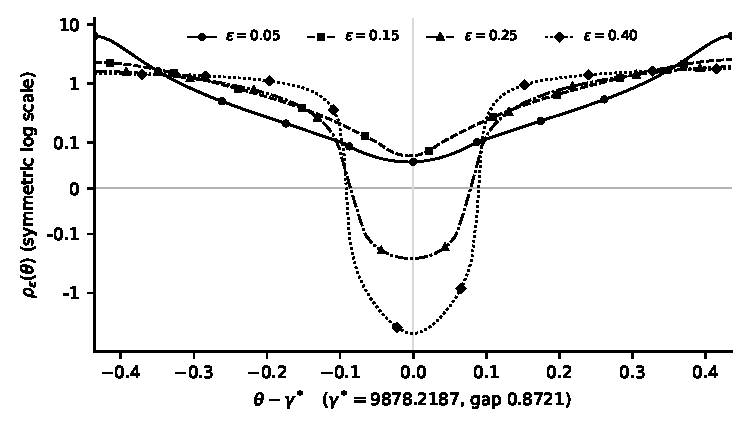
\includegraphics[width=0.82\textwidth]{fig/tf_window.pdf}
\caption{The Thorin density $\rho_\varepsilon$ across the gap at height $9878$ (gap $0.872$) with a hypothetical quadruple at distance $\delta=0.45$ inserted at its midpoint, at four levels $\varepsilon=0.05$, $0.15$, $0.25$ and $0.4$. It is positive at $\varepsilon=0.05$ and $\varepsilon=0.15$ and negative near the midpoint at $\varepsilon=0.25$ and $\varepsilon=0.4$. The vertical scale is symmetric logarithmic, linear within $\pm0.1$. Script \texttt{tf\_window.py} with the option \texttt{--plot}, data \texttt{tf\_window.json}.}
\label{tf:fig:window}
\end{figure}

\subsection{The visibility curve}\label{tf:sec:curve}

\begin{proposition}[The visibility curve]\label{tf:prop:curve}
Let $\rho^0_\varepsilon$ be the Thorin density of all zeros other than the two zeros $\tfrac12\pm\delta+i\gamma^*$ of a quadruple $\tfrac12\pm\delta\pm i\gamma^*$, so that the terms of the quadruple's images at $-\gamma^*$ are included in it (and $\delta_{\rm det}$ below depends on $\delta$ through them, by $10^{-9}$ in the computations of this section), and suppose $\rho^0_\varepsilon(\gamma^*)>0$. For $0<\varepsilon<\delta$, $\rho_\varepsilon(\gamma^*)<0$ if and only if
\[
\delta<\delta_{\rm det}(\varepsilon),\qquad \delta_{\rm det}(\varepsilon)^2=\varepsilon^2+\frac{2\varepsilon}{\pi\rho^0_\varepsilon(\gamma^*)} .
\]
In the lattice models the other zeros are those of the lattice alone, and the images at $-\gamma^*$ and the distant zeros are neglected, as in Section~\ref{sec:ch13:visibility}. Let the other zeros lie on the line at the points $\gamma^*\pm(k+\tfrac12)\Delta$ with $k\ge0$ in configuration (ii), $\gamma^*\pm k\Delta$ with $k\ge1$ in (i), and $\gamma^*\pm(k+\tfrac12)\Delta$ with $k\ge1$ in (iii). Then
\[
\delta_{\rm det}(\varepsilon)^2=\varepsilon^2+\begin{cases}
\dfrac{2\varepsilon\Delta}{\pi\tanh(\pi\varepsilon/\Delta)} & \text{in (ii),}\\[2.5ex]
\dfrac{2\varepsilon}{\frac\pi\Delta\coth\frac{\pi\varepsilon}\Delta-\frac1\varepsilon} & \text{in (i),}\\[2.5ex]
\dfrac{2\varepsilon}{\frac\pi\Delta\tanh\frac{\pi\varepsilon}\Delta-\frac{2\varepsilon}{\varepsilon^2+\Delta^2/4}} & \text{in (iii).}
\end{cases}
\]
As $\varepsilon\to0$ these tend to $\delta_c^2=2\Delta^2/\pi^2$, $6\Delta^2/\pi^2$ and $2\Delta^2/(\pi^2-8)$, and for $\varepsilon\ge\Delta$ all three satisfy $\delta_{\rm det}(\varepsilon)^2-\varepsilon^2=2\varepsilon\Delta/\pi+O(\Delta^2)$, that is $\delta_{\rm det}(\varepsilon)-\varepsilon=(\Delta/\pi)\big(1+O(\Delta/\varepsilon)\big)$. In all three, $\delta_{\rm det}$ is increasing.
\end{proposition}

\begin{proof}
The two zeros at height $\gamma^*$ contribute $\pi^{-1}\big((\varepsilon-\delta)^{-1}+(\varepsilon+\delta)^{-1}\big)=-2\varepsilon/(\pi(\delta^2-\varepsilon^2))$ at $\theta=\gamma^*$, so $\rho_\varepsilon(\gamma^*)<0$ exactly when $\pi\rho^0_\varepsilon(\gamma^*)<2\varepsilon/(\delta^2-\varepsilon^2)$, which rearranges to the stated inequality. A zero on the line at distance $\delta_j$ from $\gamma^*$ contributes $\varepsilon/(\pi(\varepsilon^2+\delta_j^2))$ to $\rho^0_\varepsilon(\gamma^*)$ (Proposition~\ref{prop:struct}), so in the lattice models $\pi\rho^0_\varepsilon(\gamma^*)=\varepsilon\sum_j(\varepsilon^2+\delta_j^2)^{-1}$, which is positive. The sum decreases with $\varepsilon$, and $\delta_{\rm det}(\varepsilon)^2=\varepsilon^2+2\big/\sum_j(\varepsilon^2+\delta_j^2)^{-1}$ increases. For the lattices, $\sum_{k\in\mathbb Z}\varepsilon/(\varepsilon^2+(k+\frac12)^2\Delta^2)=(\pi/\Delta)\tanh(\pi\varepsilon/\Delta)$ and $\sum_{k\ne0}\varepsilon/(\varepsilon^2+k^2\Delta^2)=(\pi/\Delta)\coth(\pi\varepsilon/\Delta)-1/\varepsilon$, by the partial fractions of $\tanh$ and $\coth$, and removing the two zeros at $\gamma^*\pm\frac12\Delta$ subtracts $2\varepsilon/(\varepsilon^2+\Delta^2/4)$ from the first. The limits follow from $\tanh x=x+O(x^3)$ and $\coth x=1/x+x/3+O(x^3)$, which give $\pi\rho^0_\varepsilon(\gamma^*)/\varepsilon\to\pi^2/\Delta^2$, $\pi^2/(3\Delta^2)$ and $(\pi^2-8)/\Delta^2$. For $\varepsilon\ge\Delta$, $\tanh(\pi\varepsilon/\Delta)$ and $\coth(\pi\varepsilon/\Delta)$ equal $1$ up to $O(e^{-2\pi\varepsilon/\Delta})$, so that $\pi\rho^0_\varepsilon(\gamma^*)=\pi/\Delta+O(1/\varepsilon)$ in all three, whence $\delta_{\rm det}^2-\varepsilon^2=2\varepsilon\Delta/\pi+O(\Delta^2)$; dividing by $\delta_{\rm det}+\varepsilon=2\varepsilon+O(\Delta)$ gives $\delta_{\rm det}-\varepsilon=(\Delta/\pi)(1+O(\Delta/\varepsilon))$.
\end{proof}

The first display of the proposition is the formula for $\pi\rho_\varepsilon(\gamma)$ at the ordinate in Section~\ref{sec:ch13:visibility}, solved for the distance, with all the other zeros and not only the neighbours in $\rho^0_\varepsilon$. So a level $\varepsilon$ sees, at the ordinate, exactly the zeros at distances in $(\varepsilon,\delta_{\rm det}(\varepsilon))$: a band that starts at width $\delta_c$ near the line and has width close to $\Delta/\pi=2/\log(h/2\pi)$ well above it, the scale $1/\log\gamma$ of Section~\ref{sec:ch13:visibility} with its constant. The width $\delta_{\rm det}(\varepsilon)-\varepsilon$ is $\Delta/\pi+c\,\Delta^2/\varepsilon+\cdots$ with $c=\tfrac1{2\pi^2}$, $-\tfrac1{2\pi^2}$ and $\tfrac3{2\pi^2}$ in (i), (ii) and (iii), so that for large $\varepsilon$ it is above $\Delta/\pi$ in (i) and (iii) and below it in (ii); in (i) and (iii) it falls monotonically to $\Delta/\pi$ (computed), while in (ii) it falls from $0.450\,\Delta$ to a least value $0.272\,\Delta$ at $\varepsilon=0.581\,\Delta$ and then rises to $\Delta/\pi$ from below (computed by \texttt{tf\_visibility.py}). The curve explains Table~\ref{tf:tab:window}. At the midpoint of the $10000$th gap, $\pi\rho^0_\varepsilon(\gamma^*)$ computed from $\xi'/\xi$ gives $\delta_{\rm det}(0.19)=0.4503$, and solving $\delta_{\rm det}(\varepsilon)=0.45$ gives $\varepsilon=0.1895$. Figure~\ref{tf:fig:visibility} draws the region for the actual zeros and for the lattice with the same gap, which lies within $0.015$ of it.

\begin{figure}[htbp]
\centering
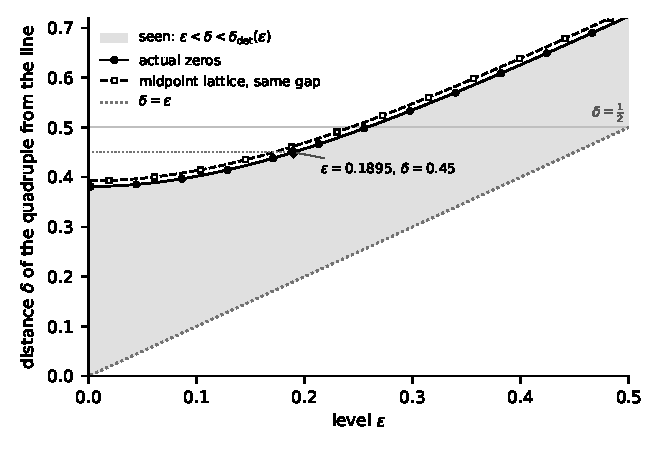
\includegraphics[width=0.82\textwidth]{fig/tf_visibility.pdf}
\caption{The visibility region $\varepsilon<\delta<\delta_{\rm det}(\varepsilon)$ (shaded band) at the midpoint of the $10000$th gap. Solid: $\delta_{\rm det}$ from the actual zeros through $\xi'/\xi$; dashed: the midpoint lattice of Proposition~\ref{tf:prop:curve} with the same gap; dotted: $\delta=\varepsilon$, the lower edge of the band. The marked point is $\varepsilon=0.1895$, $\delta=0.45$. Script \texttt{tf\_visibility.py}.}
\label{tf:fig:visibility}
\end{figure}

\begin{corollary}[How many levels, in the lattice model]\label{tf:cor:levels}
Take any of the three lattice models, with gap $\Delta=2\pi/\log(h/2\pi)$, and put $\varepsilon_1=\delta_c$ and $\varepsilon_{k+1}=\delta_{\rm det}(\varepsilon_k)$. Let $K$ be the least $k$ with $\varepsilon_{k+1}>\tfrac12$, so that $K=0$ if $\delta_c>\tfrac12$.
\begin{enumerate}
\item[(a)] The sign of $\mathcal L_\Xi(\gamma^*)$, together with positivity of $\rho_\varepsilon(\gamma^*)$ at the levels $\varepsilon_1,\dots,\varepsilon_K$, each moved down slightly so that consecutive bands overlap, detects a single off line quadruple at every distance in $(0,\tfrac12]$.
\item[(b)] No test made at the ordinate, that is the sign of $\mathcal L_\Xi(\gamma^*)$ together with the sign of $\rho_\varepsilon(\gamma^*)$ at finitely many levels, that detects a single off line quadruple at every distance in $(0,\tfrac12]$ uses fewer than $K$ levels.
\item[(c)] $K=\tfrac14\log(h/2\pi)+O(\log\log h)$.
\end{enumerate}
\end{corollary}

% CHECK: part (b) of Corollary tf:cor:levels and its proof (optimality of the greedy levels because delta_det is increasing) are written by the editor of the merge in place of the lower bound sketched in review A (finding M1, an integral of the band widths); the argument is complete but is new mathematics, to be checked by the authors. The definition of K with a strict inequality differs from the script's (least k with z_k >= 1/2) only if some iterate equals 1/2 exactly, which does not happen at the heights of Table tf:tab:levels. Detection means a strictly negative value in (a) and (b) (part (a) speaks of positivity of rho_epsilon, part (b) of the sign): if a zero value counted as detection, (b) would fail exactly when an iterate equals 1/2, for example at delta_c = 1/2 we get K = 1 although the first order test alone covers (0, 1/2]; the catalog entry defines detection strictly (review u18, last minor finding).
\begin{proof}
By Proposition~\ref{tf:prop:nearline} the first order test detects the distances in $(0,\delta_c)$, and by Proposition~\ref{tf:prop:curve} the level $\varepsilon$ detects exactly those in $(\varepsilon,\delta_{\rm det}(\varepsilon))$, since a zero at distance $\delta\le\varepsilon$ contributes positively and $\rho^0_\varepsilon(\gamma^*)>0$. Write $f=\delta_{\rm det}$, so that $\varepsilon_{k+1}=f(\varepsilon_k)$; $f$ is continuous and increasing with $f(\varepsilon)>\varepsilon$.

(a) The bands $(0,\varepsilon_1)$ and $(\varepsilon_k,\varepsilon_{k+1})$, $1\le k\le K$, cover $(0,\varepsilon_{K+1})$ except the points $\varepsilon_1,\dots,\varepsilon_K$. Moving the levels down by suitably small amounts, which is possible because $f$ is continuous and $\varepsilon_{K+1}=f(\varepsilon_K)>\tfrac12$, makes consecutive bands overlap and still reach beyond $\tfrac12$.

(b) We claim that if $j\ge1$ bands $(\varepsilon',f(\varepsilon'))$ cover $[\ell,x)$ with $\ell>0$, then $x<f^{(j)}(\ell)$, the $j$th iterate. A band containing $\ell$ has $\varepsilon'<\ell$, so its right end is $r=f(\varepsilon')<f(\ell)$. For $j=1$ this gives $x\le r<f(\ell)$. For $j>1$, either $x\le r<f(\ell)\le f^{(j)}(\ell)$, or the other $j-1$ bands cover $[r,x)$ and the claim for $j-1$ gives $x<f^{(j-1)}(r)<f^{(j-1)}(f(\ell))=f^{(j)}(\ell)$. Now suppose that $m$ levels, with the first order test, detect every distance in $(0,\tfrac12]$. The point $\delta_c$ is not in $(0,\delta_c)$, so unless $\delta_c>\tfrac12$ (and then $K=0$) some bands cover $[\delta_c,\tfrac12]$, and the claim with $\ell=\delta_c$ and $x=\tfrac12$ gives $\tfrac12<f^{(m)}(\delta_c)=\varepsilon_{m+1}$. By the definition of $K$, $m\ge K$.

(c) The bands advance by $a(\varepsilon)=\delta_{\rm det}(\varepsilon)-\varepsilon=\big(\delta_{\rm det}(\varepsilon)^2-\varepsilon^2\big)/\big(\delta_{\rm det}(\varepsilon)+\varepsilon\big)$, which by the formulas of Proposition~\ref{tf:prop:curve} is $\frac\Delta\pi\big(1+O(\Delta/\varepsilon)\big)$ for $\varepsilon\ge\Delta$ and, for $\varepsilon\le\Delta$, lies between two positive constants times $\Delta$, since $a(\varepsilon)/\Delta$ is a positive continuous function of $\varepsilon/\Delta$. The number of steps from $\delta_c$ to $\tfrac12$ is therefore $\int_{\Delta}^{1/2}\frac{d\varepsilon}{a(\varepsilon)}+O(\log(1/\Delta))=\frac\pi\Delta\big(\tfrac12+O(\Delta\log(1/\Delta))\big)$, and $\pi/(2\Delta)=\tfrac14\log(h/2\pi)$, while $\log(1/\Delta)=O(\log\log h)$.
\end{proof}

\begin{table}[htbp]
\centering\footnotesize
\begin{tabular}{@{}rcccc@{}}
\toprule
$h$ & $\tfrac14\log(h/2\pi)$ & (i) replacing & (ii) midpoint & (iii) count preserving\\
\midrule
$10^{5}$ & $2.4$ & $0$ & $2$ & $0$\\
$10^{8}$ & $4.1$ & $2$ & $4$ & $1$\\
$3\times10^{12}$ & $6.7$ & $4$ & $6$ & $3$\\
$10^{22}$ & $12.2$ & $9$ & $12$ & $7$\\
\bottomrule
\end{tabular}
\caption{The number $K$ of greedy levels of Corollary~\ref{tf:cor:levels}, counted without the downward moves, in the three lattice models with $\Delta=2\pi/\log(h/2\pi)$, against $\tfrac14\log(h/2\pi)$. Script \texttt{tf\_visibility.py}.}
\label{tf:tab:levels}
\end{table}

Table~\ref{tf:tab:levels} gives the numbers of levels. The count preserving lattice has the larger $\delta_c=1.034\,\Delta$, which stays above $\tfrac12$ up to $h=2.8\times10^6$, so it uses fewer levels, and at $10^5$ the $\delta_c=0.506$ of the replacement lattice already covers every distance. At the height $3\times10^{12}$ to which RH has been verified~\cite{PT21} the three models use between three and six levels. The corollary is a statement about a model with a single quadruple and regularly spaced neighbours, and about tests at the ordinate: a test that looks for negative values anywhere in the window can see more (Section~\ref{sec:ch13:visibility}, Exercise~\ref{ex:ch15:beside}), and for it no lower bound is proved here. Turning it into a certificate for the actual zeros is Problem~\ref{tf:prob:levels}.
